
\chapter{Implementation}
\label{chap:implementation}
This chapter describes the implementation of our social networking site, the User Interface and how the system scales.

The system consists of the following components, as shown in figure~\ref{fig:system_architecture}: In the first layer lives (1) the Social Networking engine, which runs all PHP scripts, as described in section~\ref{sec:implementaion_of_social_netowrk}. 
In the second layer lives (2) the Memcached caching system, which described in section~\ref{sec:memcache_implementation}. 
In the third layer lives (3) the Social Network MySQL database, and (4) the CDO server - client components as well as the CDO repository. The Social Networking Engine at layer 1 is defined as the front end system and the CDO Client, the memcached nodes, the CDO Server and the repositories are defined as the back end system. 

\begin{figure}[h]
	\caption{The overall architecture of Social Network.}
	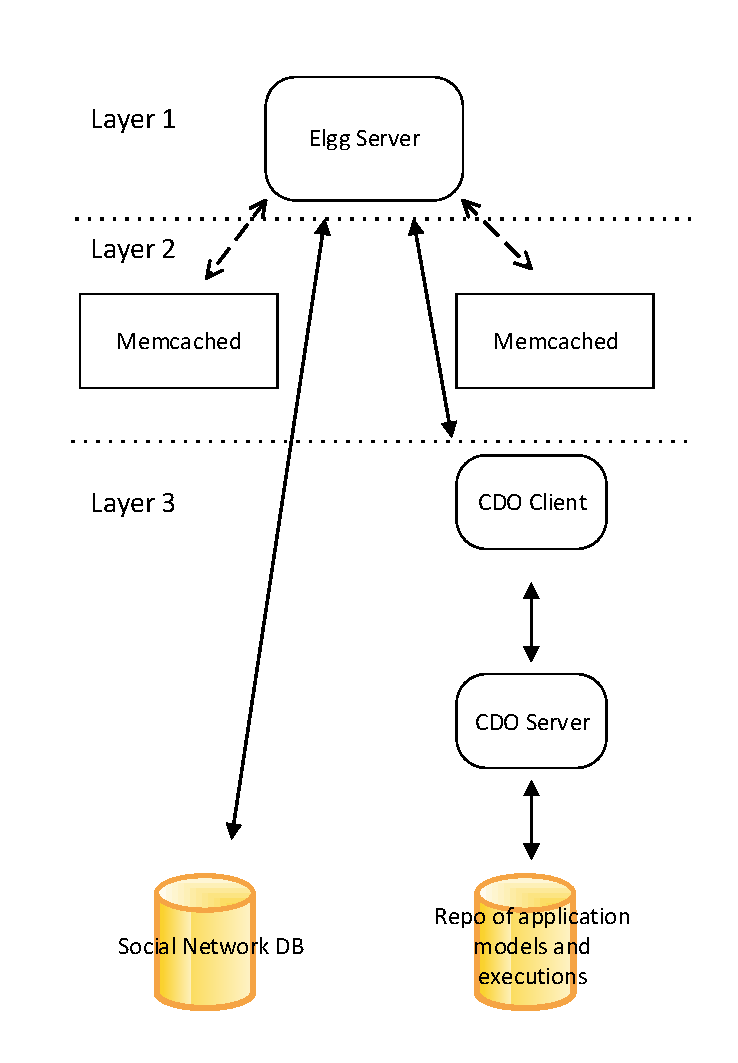
\includegraphics[width=0.6\textwidth,natwidth=200,natheight=150]{./fig/system_architecture.pdf}
	\centering
	\label{fig:system_architecture}
\end{figure}

In order to achieve the scalability of the system, two system architectures are examined at two layers of the system: (1) We added more than one Social Network engines at the first layer of the system. In this implementation, in order to keep the file system in consistent mode we integraded Apache Zookeeper~\cite{zookeeper_url} as described in section~\ref{sec:engine_scale}. (2) We added more than one memcached nodes at the second layer in order to add more cpu capacity and improve the system's response time as described in section~\ref{sec:memcache_implementation}.

\section{Implementation of Social Network}
\label{sec:implementaion_of_social_netowrk}
The social networking platform is implemented over the extensible Elgg social network framework~\cite{elgg_url}.  Elgg is an open source software written in PHP, that uses MySQL for data persistence and supports jQuery~\cite{jquery_url} for client-side scripting.  

The overall architecture of Elgg Social Network is shown in figure ~\ref{fig:elgg_architecture}. The Elgg Social Network is structured following the key concepts of Model-View-Controller (MVC) known architectural pattern for User Interfaces. The MVC system is analyzed here, depicting the most important aspects of it from the Elgg's perspective. Explaining the Elgg's architecture by using MVC system will make the understanding of Elgg less complex.

Figure~\ref{fig:elgg_architecture} shows the model, view, and controller parts of Elgg's architecture. In a typical scenario, a web client requests an HTML page (e.g., the description of an application model).  The request arrives at the \emph{Controller}, which confirms that the application exists and instructs \emph{Model} to increase the view counter on the application model object. The controller dispatches the request to the appropriate handler (e.g., application model, component handler, community handler) which then turns the request to the view system. View pulls the information about the application model and creates the HTML page that is returned to the web client.

The {\bf Model} of the framework is structured around the following key concepts as shown in figure ~\ref{fig:elgg_entities}:
\begin{itemize}
\item \emph{Entities}, classes capturing social networking concepts: users, communities, application models. Elgg Core comes with four basic objects: ElggObject, ElggUser, ElggGroup, ElggSite, ElggSession, ElggCache and a lot of other classes necessary for the proper engine operation.
\item \emph{Metadata} describing and extending entities (e.g., a response to a question, a review of an application model, etc.).
\item  \emph{Relationships} connect two entities (e.g., user A is a friend of user B, user C is a contributor to an application model, etc.) and are persisted in the Social Network DB.
\item \emph{Annotations} are pieces of simple data attached to an entity that allow users to leave ratings, or other relevant feedback.
\end{itemize}

\begin{figure}[h]
	\caption{Architecture of the Elgg Social Networking engine.}
	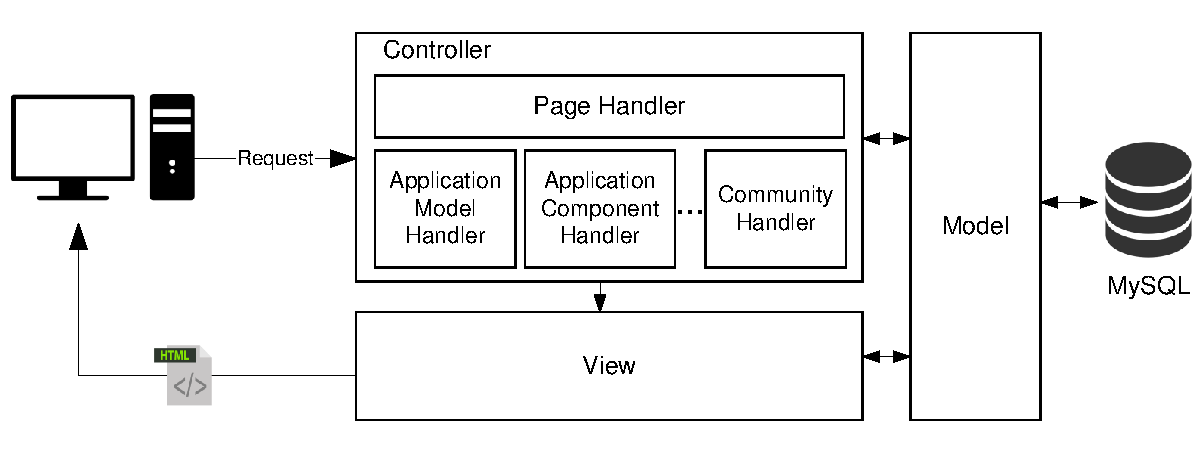
\includegraphics[width=0.9\textwidth,natwidth=200,natheight=150]{./fig/elgg_architecture.pdf}
	\centering
	\label{fig:elgg_architecture}
\end{figure}

All Elgg objects inherit from ElggEntity, which provides the general attributes of an object. Elgg core comes with the following basic entities: ElggObject, ElggUser, ElggGroup, ElggSite, ElggSession, ElggCache, as well as other classes necessary for the operation of the engine.

\begin{figure}[h]
	\caption{The Elgg Engine Data model.}
	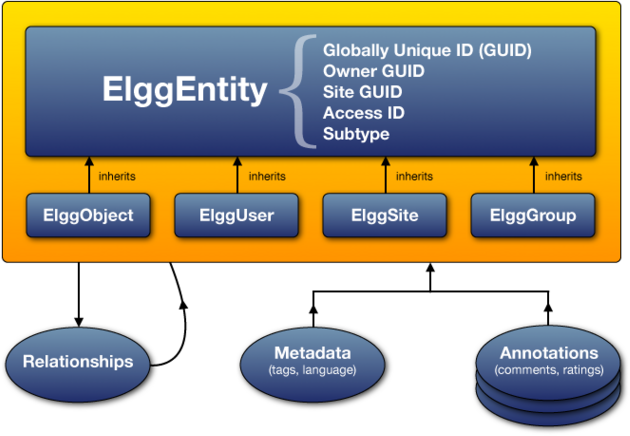
\includegraphics[width=0.6\textwidth,natwidth=200,natheight=150]{./fig/elgg_data_model.png}
	\centering
	\label{fig:elgg_entities}
\end{figure}

The {\bf controller} component of MVC model of Elgg consisting of the \emph{Actions} of the system which are the primary way the users interact with the Elgg site. An action in Elgg Framework is the code that make changes to the database when a user performs an action like logging in, posting a comment, or creating an application model. The action script processes input, makes the appropriate modifications to the database, and provides feedback to the user about the action. By default, actions are only available to logged in users and include Cross-Site Request Forgery (CSRF) Security token to overcome session fixation~\cite{kolvsek2002session}, Session Hijacking~\cite{burgersposter} and Cross-site Scripting~\cite{thamescomparing}.

Additionally, the controller component includes the \emph{Events} and the \emph{Plugin Hooks}, which are used in Elgg Plugins to interact with the Elgg engine. Events and hooks are triggered at important times throughout Elgg’s boot and execution process, and allows plugins to modify or cancel the default behaviour of Elgg. When an event is triggered, a set of handlers is executed in order of priority. Each handler passes the arguments and has the option to influence the process. When the execution of the current handler is completed, the ``trigger'' function returns a value based on the behaviour of the handlers.

The {\bf View} component is responsible for creating the output. Generally, this will be HTML sent to a web browser, but it could also be XML, JSON or any other data formats. View handles everything from the layout of pages and chunks of presentation output (like a topbar ) down to individual links and form inputs.

Elgg comprises a core system that can be extended through plugins (examples are the Cart system and the handling of Application Models). Plugins add new functionality, can customize aspects of the Elgg engine, or change the representation of pages.
A plugin can create new objects (e.g., ApplicationObject) characterized (through inheritance of ElggEntity) by a numeric globally unique identifier (GUID), an owner GUID and an Access ID. Access ID encodes permissions ensuring that when a page requests data it will not touch any data the current user does not have permissions on. All plug-ins share a common structure of folders and PHP files, following the MVC model of figure~\ref{fig:elgg_architecture}.  

The hierarchy of a plug-in is shown in figure~\ref{fig:elgg_hierarchy}. 
The folder {\em actions} includes the actions applied on application models. Every active participation of the user is performed via an action. Logging in, creating, updating or deleting content are all general categories of actions.
The {\em views} folder contains the {\em php} forms applied on application models, {\em river} events (Elgg terminology for live feeds). Viewss are responsible for creating the output for the client browser. Generally, this will be HTML, but it can be also JSON or other format. 
{\em Pages} overrides elements of core Elgg pages and can be from chunks of presentation output (like sidebars) down to individual html code.  
The {\em js} and {\em lib} folder provides javascript and {\em php} library functions. 
Finally, the {\em vendors} folders include third-party frameworks such as Twitter's bootstrap front-end~\cite{bootstrap_url}.
The most important file of a plug-in is the \emph{start.php} script, which contains the \emph{page handler}. Page handler is a function manages the plug-in pages enabling custom url redirect to a specific page. 
The plug-in initialization is also defined in the start.php and registers actions, events and determines the views. 

\begin{figure}[h]
	\caption{The structure of the application description plug-in.}
	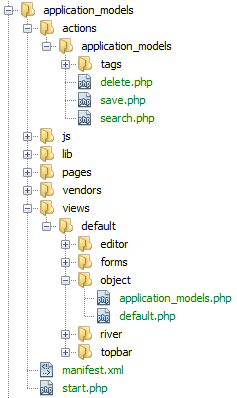
\includegraphics[width=0.4\textwidth]{./fig/folder_hierarchy.png}
	\centering
	\label{fig:elgg_hierarchy}
\end{figure}

Finally, as mentioned before, for client side scripting the jQuery is used. The main reason why jQuery is preferred in this work over of pure JavaScript~\cite{mccormick2004jquery} is that it's a light library which pushes content to the client machine, it therefore reduces the wait time for server response. Plus, it's smaller than Flash, so it results in smoother playbacks and less errors. Furthermore, jQuery works anywhere since is cross-browser compatible with any browser, mobile phone or tablet, and Apple devices. Finally, another hand-solving advantage of jQuery is its simple syntax.It is designed to make it easier to navigate in a document, select HTML DOM elements, create animations, handle events, and developing Ajax applications. 

Thus, the jQuery is used by SNP for implementing client side scripting and for the remaining of this chapter, when we refer to JavaScript, we actually refer to the jQuery library. 
Furthermore, some other JavaScript libraries are used in order to make the User Interface more powerful. One of those libraries is the Chart.js~\cite{chartjs_url} library which is used to generate the graphs and charts in execution's page.

\subsection{New functionality of Elgg Social Network Platform}
As described in the previous section, the new functionality of Elgg Social Networking Platform can be introduced by new plugins. Since the modification of the core system is not a good practice, because it makes the system more difficult to implement and does not let it upgrade to the new versions of Elgg framework. The following plugins are implemented:

\textbf{ApplicationModel}. The ApplicationModel plugin has a {\it page handler} to manage the application Model pages. Also, ApplicationModel has client side JavaScript for manipulating User Interaction and dynamic pages. Furthermore, some php libraries are implemented, for example a library for interaction with CDO client or a library for manipulating Application models. 

\textbf{Components}. The Components plugin has a {\it page handler} to manage the Components pages and their Categories and a PHP library to interact with Chef supermarket.

\textbf{CustomView}. The CustomView plugin has all the necessary customization of the PaaSage Social Networking Platform (PSNP). All custom views of the system are implemented in this plugin. This plugin overrides all the default views of the Elgg that should be changed and contains client side JavaScript. Furthermore, CustomView has the following seven page handlers: {\t profile} responsible for profile pages, {\t avatar} responsible for the photos of user pages, {\t settings} responsible for the pages of user settings, {\t friends} responsible for the friends of the user pages, {\t contact} responsible for the Contact Information of the PSNP, {\t review} responsible for the reviews of Application Models and {\t search} responsible for the main search facility of PSNP. Finally, CustomView has all the required \emph{Actions} of the plugin such as the vote up or down, the action to add a review etc.

\textbf{NotificationSystem}. This plugin is responsible for the notifications of the Social Network which contains a relevant page handler, JavaScript for client side scripting and a php server side library.

\textbf{Tags}. This plugin does not include any page handlers but only the necessary actions for the Tags such as {\it add} or {\it delete} a Tag and a php library responsible for those. 

\textbf{UserStatistics}. This plugin is responsible for collecting and displaying the information about the Users.

\textbf{Memcached}. This plugin has all the essential functionality for memcached implementation as will be described in section~\ref{sec:memcache_implementation}.

\textbf{ZookeeperRecipes}. This plugin has all the essential functionality for memcached implementation as will be described in section~\ref{sec:engine_scale}.

\textbf{Groups}. The Groups plugin is the default plugin of Elgg Framework modified to support the required functionality.

\textbf{Messages}. The Messages plugin is the default plugin of Elgg Framework modified to support the required functionality.

\subsubsection{Twitter bootstraping of Elgg}
Responsive Web design (RWD)~\cite{natda2013responsive} is a Web design approach aiming at crafting web application sites to provide an optimal viewing experience, which it provides easy reading and navigation with a minimum of resizing, panning, and scrolling, across a wide range of devices (from mobile phones to desktop computer monitors). However, the default CSS of Elgg, which is part of the View component of architecture, does not offer responsive web pages. Thus the ideal solution is to integrate Twitter Bootstrap to Elgg Viewing System. 

Twitter Bootstrap~\cite{twitter_bootstrap}~\cite{cochran2012twitter} is a free and open-source collection of tools for creating dynamic websites and web applications. It contains HTML and CSS-based design templates for typography, forms, buttons, navigation and other interface components, as well as optional JavaScript extensions. It aims to ease the development of dynamic websites and web applications. 

We customize the Elgg View inserting the Twitter Bootstrap View System. The default View System of Elgg changed to support the Twitter Bootstrap responsive grid.

\subsection{CDO communication with Social Networking Platform}
\label{sec:cdo_comm}
As mentioned in~\ref{sec:background}, the execution history of deployments of application models and the description of those models are stored in the CAMEL information repository, which is implemented as an Eclipse CDO server. In order to communicate with the CDO Server, a CDO Java Client is needed. The CDO client stands between the Social Networking Engine (Elgg Server) and the CDO server, making the exchange of information between those two possible, as shown in figure~\ref{fig:system_architecture}.

Specifically, regarding the communication between the CDO Server and the Client, the CDO Client opens one or more sessions to the CDO Server. Each session represents a connection to the CDO repository and provides a broad API to interact with it. A session does not provide direct access to model instances; views or transactions are needed in order to navigate or modify the model instance graph. The implemented CDO Client exposes read/write access to the repository for either viewing the execution histories or the model of the applications, or for storing new execution models. For the communication between the Social Networking Engine and the CDO Client, the CDO Client exposes a RESTful API to the Social Networking engine providing all the necessary methods. 

For example, when a user from the Social Network requests the execution histories of an application, the Engine sends a request to the CDO Client through the RESTful API, the CDO Client receives the request and forwards an appropriate request to the CDO Server. The CDO Server receives the request and queries the Repository of Application models and executions. When the CDO Server receives the response, it forwards the response back to the CDO Client, which forwards the response back to the Social Networking Engine. The Social Networking Engine transforms the response to JSON format, in order for it to be readable by the JavaScript. JavaScript plays the final role, by projecting the execution histories in a proper table to the end user that requested the page of the executions of an application.

\section{Scaling Social Network Engine}
\label{sec:engine_scale}
This section describes how the horizontal scale of Social Network engine is achieved by adding more than one Elgg Servers. At the layer 1 of figure~\ref{fig:elgg_architecture} lives the Apache2 server, which as the stress test of the system indicates in chapter~\ref{chapt:evaluation}, takes a heavy load on CPU utilization. 

The heavy load of Apache2 server occurs by the nature of Elgg Framework. Because the Elgg core system is implemented to be extensible and configurable, every time a simple page or just an AJAX call is received by the Elgg, the Elgg Framework performs the following heavy tasks: it broadcasts an {\it init system} event; this event is caught by all plugins of Elgg and at this initialization phase the plugins register: (1) the page handlers, (2) the PHP libraries, (3) the actions, (4) the events and hooks, (5) the JavaScript libraries and (6) the CSS scripts. Therefore, all those actions generate a heavy load resulting in consuming CPU utilization and slowing the response time of the system. We introduce more than one Apache2 Servers running the Social Networking Engine of Elgg Framework to overcome this.  

The Social Networking Engine keeps some information in the file system instead of in the Social Network Database. This information includes the profile photos of users and any other images such as photos that users add to the community groups. Furthermore, the initial configuration of Social Networking Engine keeps in the file system some caching files. Those files represent some views of the web pages which are independent of any specific users and remain unchanged among all users. This file system caching feature is removed from the Social Network Engine because it is more efficient to use memcached for the caching instead of the slow file system.

In order to all SN Engines have access to the same file system, the Network File System (NFS)~\cite{sahni2015network} is used. NFS allows a server to share directories and files with clients over a network. With NFS, users and programs can access files on remote systems as if they were stored locally.

In our implementation, NFS is configured and used in order to allow all Social Networking Engines to gain access to the same file system store. An NFS server is installed in one of the SN Engines and all the other SN Engines have an NFS client accessing the remote file system.   

Distributing Social Network Engine was not an easy problem to solve, so Apache ZooKeeper~\cite{zookeeper_url} is used. 
Apache ZooKeeper~\cite{hunt2010zookeeper} is a service for coordinating processes of distributed applications. Since
ZooKeeper is a part of a critical infrastructure, it aims to provide a simple and high performance kernel
for building more complex coordination primitives at the client. 
We use this service in order to enable highly reliable distributed coordination among the file system and the Social Networking Engine. 
Apache ZooKeeper provides a tree abstraction where every node in that tree (or znode) is a file on which a variety of simple operations can be performed. ZooKeeper orders operations on znodes so that they occur atomically. Therefore there is no need to use complex locking protocols to ensure that only one process can access a znode at a time. The tree represents a hierarchical namespace, so that many distinct distributed systems can use a single ZooKeeper instance without worrying about their files. 

Social Networking Engine uses Apache ZooKeeper in order to keep the file system consistent, in rare but possible scenarios like two users trying to upload a file to the same group simultaneously. When a Social Networking Engine wants to write a file in file system, it first locks the specific path and after finishing the write operation it releases the lock. Thus, a file can never be corrupted.

For communication between the Apache ZooKeeper and the Elgg framework, the php-zookeeper-recipes~\cite{zookeeper_recipes_url} are used by the ZookeeperRecipes plugin. Specifically, the {\it exclusive locks} of Zookeeper are used to keep the system in consistent mode.

\section{Memcached}
\label{sec:memcache_implementation}
This section describes how we integrated and impemented memcached~\cite{memcache_url} to our system architecture. Memcached is an open source, high-performance, distributed memory object caching system. We chose memcached, because it is a generic simple in-memory key-value store. It has a powerful API available for PHP. After memcached integration the system decreased its response time and its performance.

Memcached is added in layer 2 of the system architecture as shown in figure~\ref{fig:system_architecture} and is used for storing the key-value tuples. The following data are stored in Memcached: 
\begin{enumerate}
\item MySQL responses, which are values from Social Network Database such as entities of Social Network, applications, components, users, group discussions. By storing those values, there is no need to query the Social Network Database, but SN Engine is getting the key-values directly from Memcached.
\item Views of the web pages which are independent of any specific users and remain unchanged among all users, and werte previously were stored in the file system.
\item JavaScript code results. Some JavaScript code is time consuming to be generated. For example, PHP sends the execution data to JavaScript and then it iterates the data in order to generate the tables and the graphs of execution histories.
\item Executions histories from repository of application models. By storing the executions of applications at Memcached, the system's response time decreases. That is due to the PHP modules not needing to go through the heavy CDO client-server communication but them getting the executions of applications directly from Memcached.
\end{enumerate}

The keys stored in Memcached must be unique. This is implemented using as a prefix of the key the globally unique identifier (GUID), generated by Elgg, and a string value which is describing the data. So, the execution data of an application model with QUID 1000 is stored in memcached with key {\it 1000:execution-data} and the value is the json representation of those data. All tuples at Memcached are inserted with the maximum key expiration time of thirty days.

\begin{figure}[h]
	\caption{The scenario (a) depicts a request from memcached when the key does not exist and scenario (b) depicts an updated operation of a value}
	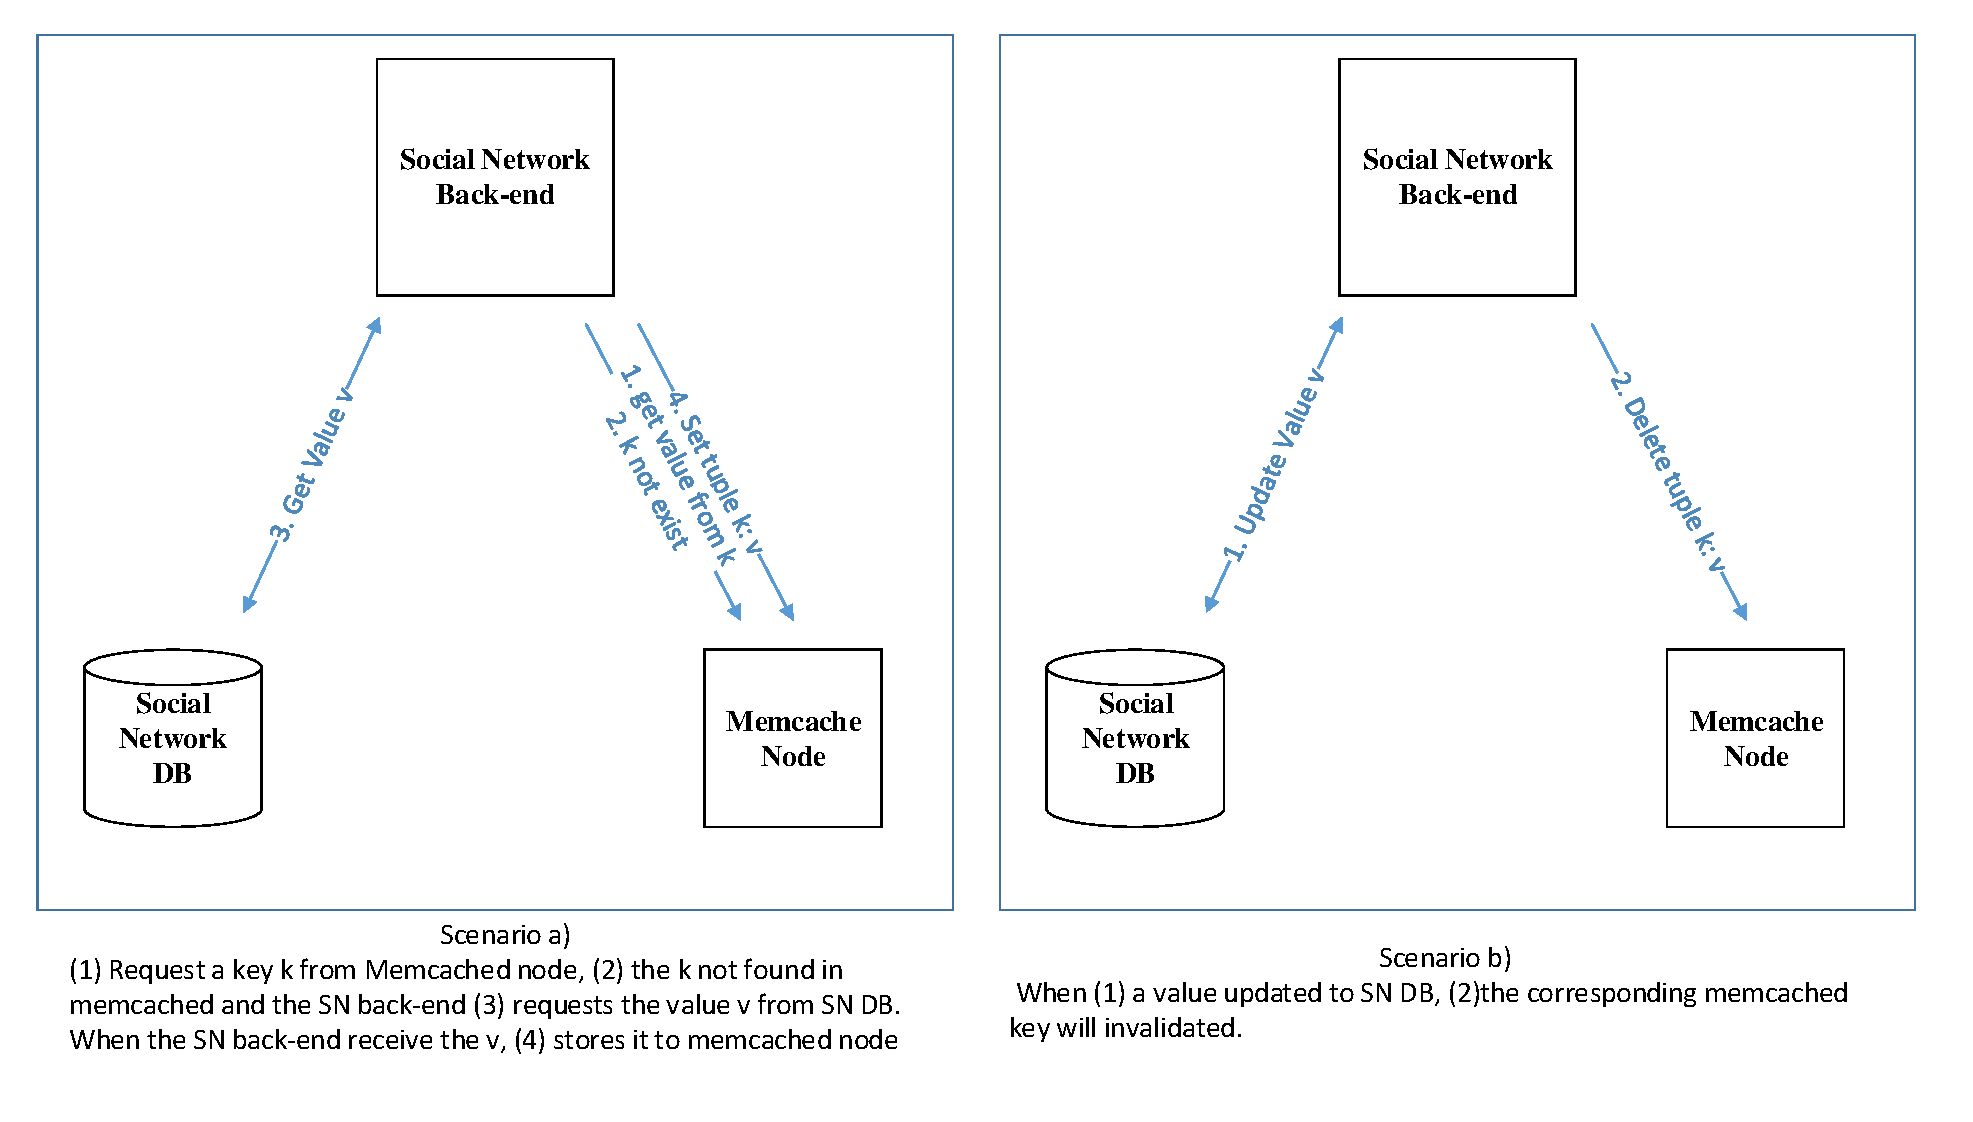
\includegraphics[width=1\textwidth]{./fig/memcached_key_value.pdf}
	\centering
	\label{fig:memcache_key_value}
\end{figure}

The basic actions of Memcached are the get, set and delete of a tuple, as shown in figure~\ref{fig:memcache_key_value}. In the first scenario, when a value from SNP is requested for a particular key {\it k}, first a query will be send to Memcached requesting the tuple with that key {\it k}, if {\it k} not found or it has expired, the SNP will request that key from the Social Network Database. Finally, when SNP gets in touch with the data of the key, it will send those data to be cached in Memcached, as shown in the figure~\ref{fig:memcache_key_value}a. In the other scenario, when a value in the SNP is updated, the memcached key will be deleted(invalidated) as shown in the figure~\ref{fig:memcache_key_value}b.

The Elgg Framework comes with the potential use of memcached but is restricted to the fact that a memcached node must be in the same machine as the Elgg Framework. Plus, it makes it more difficult to configure when an insertion in memcached node will take place. Therefore, a new Elgg plugin is implemented called \textbf{Memcached} using the memcached PHP library~\cite{memcached_php_doc}. The basic memcached functions offered by this plugin are: (1) Add memcached nodes, (2) add a key to a node, (3) get a value of a key and (4) delete a key-value item. 

The Apache JMeter~\cite{jmeter_url} was used to measure the response time of the system and the sysstat tool~\cite{sysstat_url} was used to measure the CPU usage. Section~\ref{sec:eval_memcache} 
 shows the performance results of this implementation.

\section{Natural Language Processing and classification}
\label{sec:natural_implementation}
Natural Language Processing(NLP)~\cite{manning1999foundations} is a feature added to the Social Network Platform. NLP is used in the interactions between the users and the SNP, in the way the platform can understand and determine the type of user input. 

As the figure~\ref{fig:auto_classification} shows, a user of SNP poses a question to our platform. The platform can process the user's input and classified into: (1) a similar question that exists in our community or (2) an automated generated query to the CAMEL repository. In the first scenario, a list of answers from the pre-existing question can be provided as feedback to the new question. In the second scenario, the question can be further processed and automatically generate a query to CAMEL repository. An automated mechanism can be implement for the second scenario but this is out of the scope of this thesis.  

\begin{figure}[h]
	\caption{Classification of questions and automated feedback to user}
	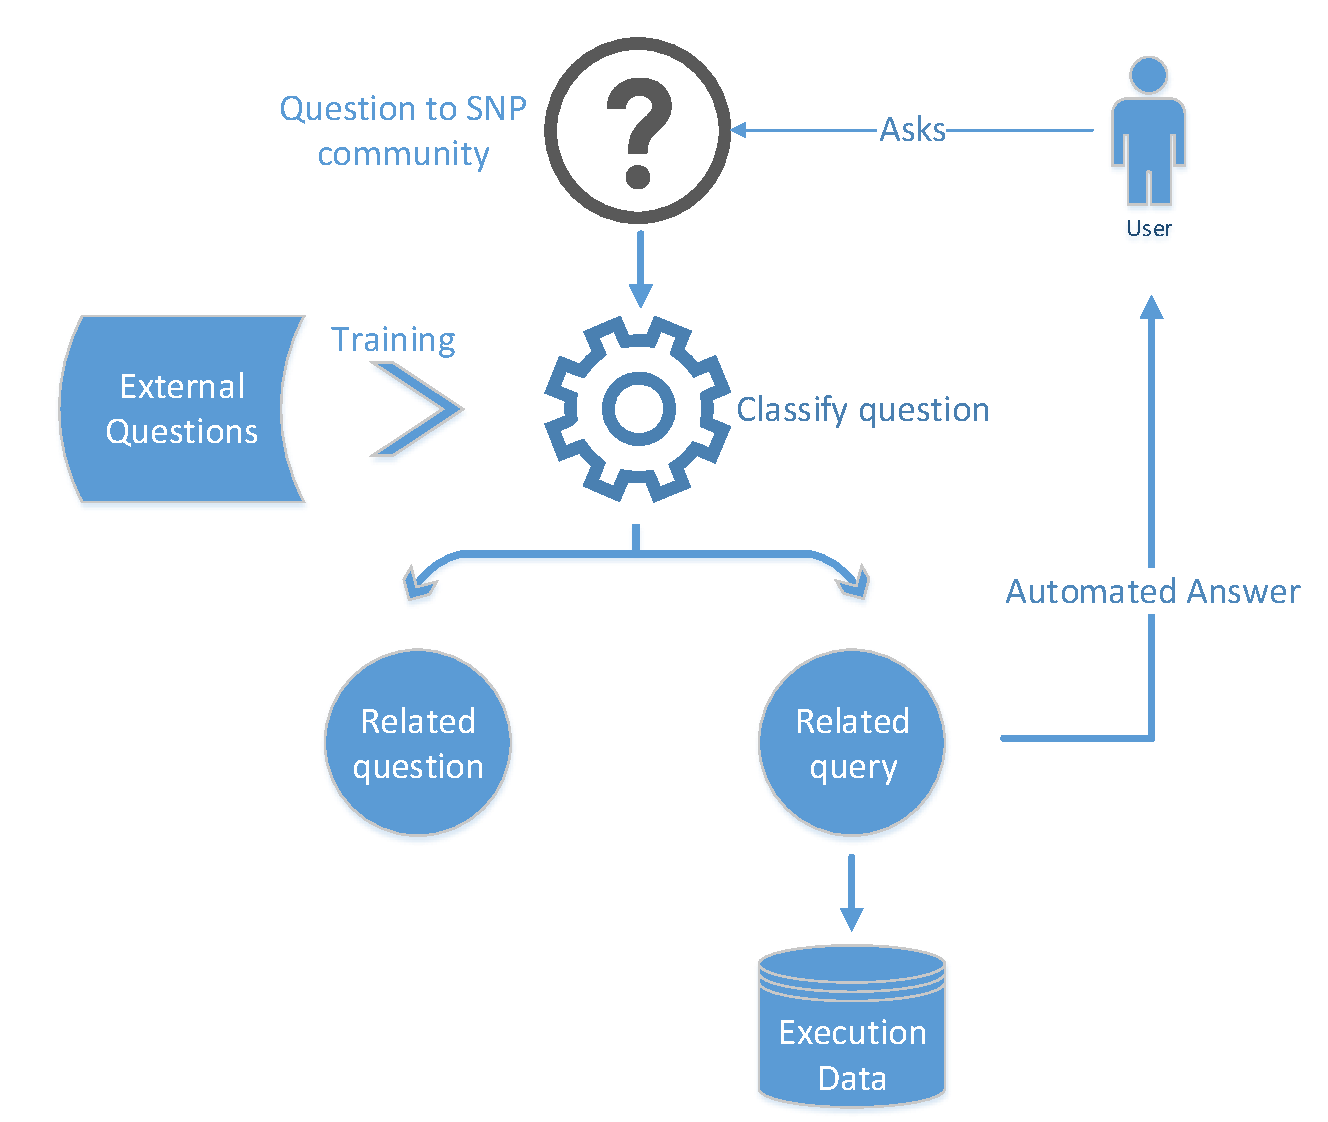
\includegraphics[width=1\textwidth]{./fig/Decision_making.pdf}
	\centering
	\label{fig:auto_classification}
\end{figure}

Our implementation is in-between of those two scenarios. Some queries to the CAMEL repository is implemented and if a question asked and in a way talk about this specific query, the Platform will provide this query's results as an answer to the user's question. Furthermore, if this question has a similar question and that last question has an answer from a sophisticated user, who had created an hand-crafted query to the repository and had provided the results back to the user. Those results can be used as a feedback to the new question. 

Particularly, Naivy Bayes Natural Language Understanding algorithm is added to the SN using the Natural framework~\cite{nodenatural_url} implemented with node.js. In general, Machine Learning algorithms such as Naivy Bayes, want an input, called data set, of training data. This training data is pulled from questions users post in StackOverflow (SO). Those questions are an excellent repository to train the NB algorithm, because they are categorised by tags and because by the time that this implementation took place, the Social Network did not include a big variety of questions in the repository.

In general, the main actions that SO users is shown in figure~\ref{fig:stackoverflow_questions}. When users ask questions in SO, they must specify some tags describing their questions. A tag is a keyword or a label that places their question in a category with other, similar questions. The users of SO sometimes, try to add as many tags as possible in order to make their questions popular and get them answered. SO permits the users to add up to only five tags in each of their questions. After a question is posed, the whole community of SO can vote the question up or down and the privileged users can flag the question as \emph{duplicate}, \emph{off-topic}, \emph{unclear}, \emph{too broad} or \emph{primarily opinion-based}. This way, low quality questions will be removed from the site resulting in keeping the questions repository clear and helpful for other potential developers to use.

For the training sets, the data to train the NB algorithm, the most voted questions of the SO community are used. Those questions have emerged as the best questions in their field and surely, we avoid the case of using a training set with miss-tagged questions that would result a miss-guided NLP classification. The NLP training set is retrieved from SO site using the stack exchange(SE) API~\cite{stackexchange_url}. The SE API is a powerful API, which allows us to take the questions, the answers, the users and all the information that exists in SO site through a programming interface.

\begin{figure}[h]
	\caption{The main StackOverflow users' actions and NLP Classifier. }
	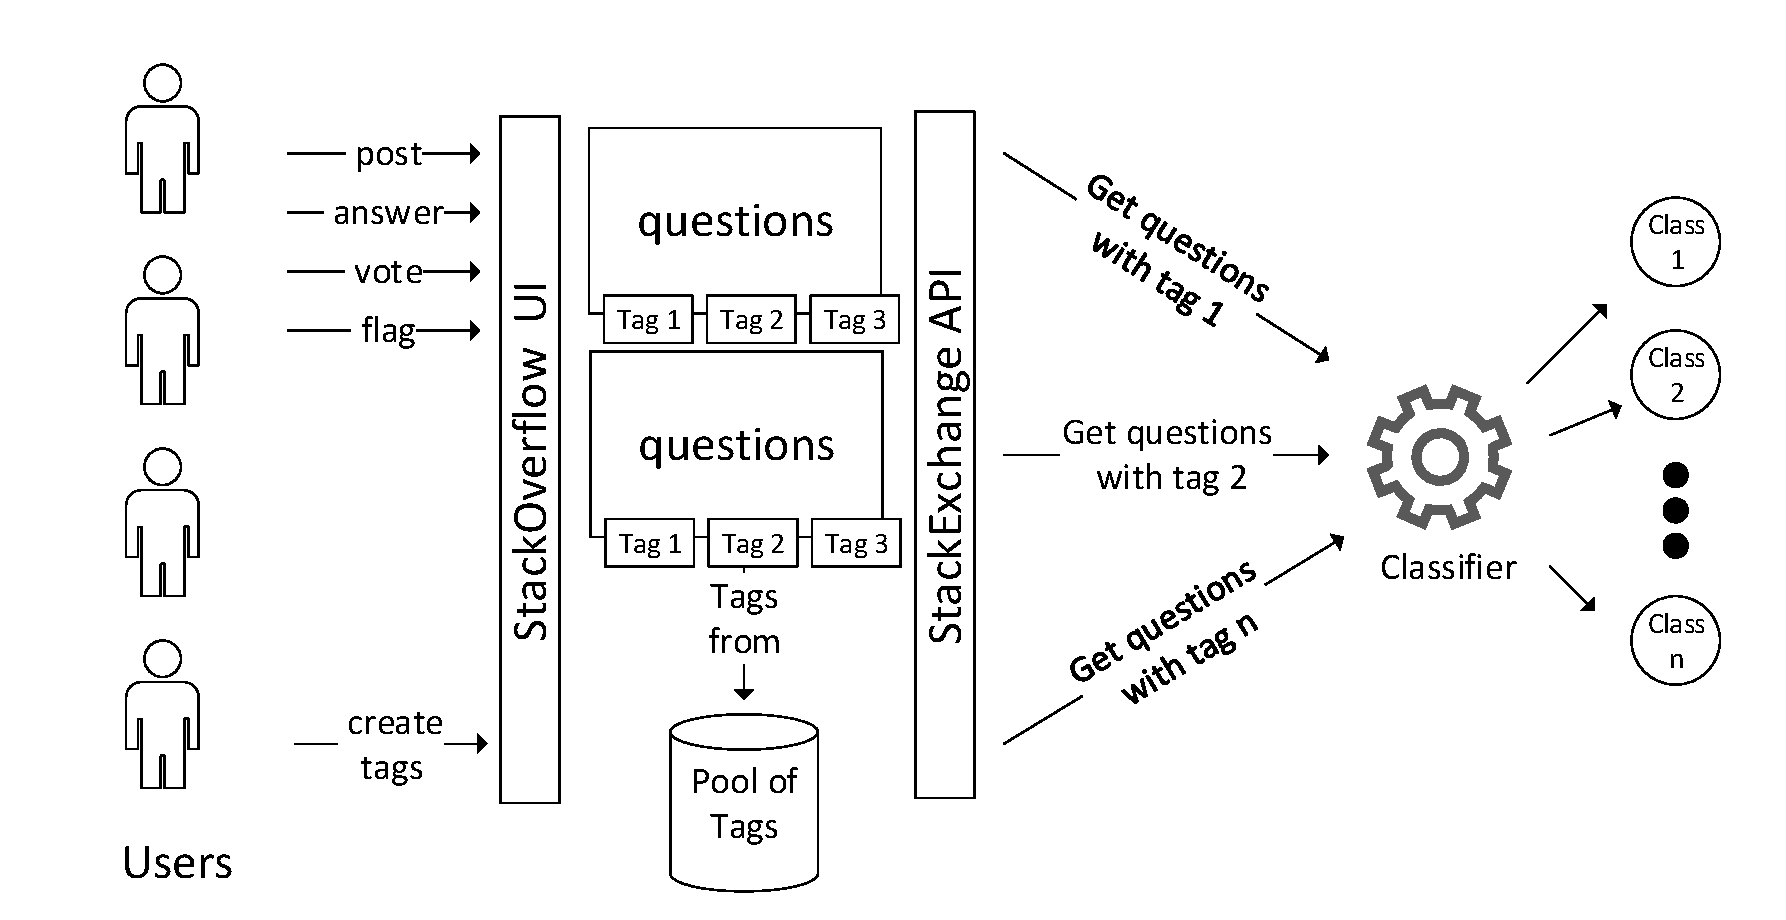
\includegraphics[width=1\textwidth]{./fig/StackOverFlow.pdf}
	\centering
	\label{fig:stackoverflow_questions}
\end{figure}

The first training set of our Natural Processing Tool consisted of five tags, relative to our platform. Those tags were: \emph{scalability}, \emph{reliability}, \emph{design}, \emph{performance} and \emph{optimization} and we got thirty questions per tag. For each of the tags, the thirty most up-voted questions from StackOverflow were retrieved and classified to each specific tag. Those exact tags, after classification, are transformed in classes in NLP classification, as shows the figure~\ref{fig:stackoverflow_questions}

Every time a user asks a question to one of the platform's communities, the classifier determines the class of the question. After the class is found, and if the platform is able to determine a heuristic answer, it will post then the answer to the user's question automatically. All the users of the platform can vote this answer up or down, depending on its accuracy, or provide their own answers.

The second training set of Natural Processing Tool was retrieved by automatically discovering tags. NB is trained with ten thousand (10000) questions from StackOverflow Q\&A site, fifty questions per each discovered tag. The general algorithm is shown below. Firstly, the algorithm starts with a tag that is relevant to the Social Network Platform such as \emph{scalability} at line 01. Afterwards, using the SE API the algorithm gets the 5 most voted questions tagged with \emph{scalability}. For each question (line 04), the populateClassifier clears the body from any html tags inserted by the StackOverflow users to beatify their questions (line 05) and classifies this question's body with each tag. Automatically, the populateClassifier proceeds to the next tag of this question. When the populateClassifier is finished the NB is trained. It should be noted that a question may have more than one tags, so a question can be classified to up to five tags / classes. Changing the threshold parameter at the following algorithm, the \emph{populateClassifier} can classify questions with an arbitrary number of tags. At the following section the process to Bayes classification is described in more details.

\begin{lstlisting} 
01:var tags = ['scalability']
02:populateClassifier(0)
03:function populateClassifier(index) {
04:  var questions = stackexchange.api.getQuestionsByTag(tags[index])
05:  foreach(questions as q)
06:    body = clear(q.body)
07:    foreach(q.tags as t)
08:    	 classify(body, t)
09:    	 if(not tags.exist(t) and tags.length() < threshold)
10:    	   tags.push(t)	  
11:        populateClassifier(tags.indexOf(t))
12:}		
\end{lstlisting}

\subsection{Bayes Classification Algorithm}
In this section the Bayes classification algorithm will described. As the above code snippet shows at line 08, the algorithm classifies a document named \emph{body} into the class \emph{t}. This \emph{body} is the content of the question that will be classified into the class \emph{t}, which is the tag of the question. Diving in this function, the \emph{body} is transformed to lower case and the Porter Stemming Algorithm~\citep{porter1980algorithm} is used for suffix stripping, so the plural form of the words and the suffixes are removed (such as \emph{-ing} and \emph{s}). For example, the following words: {\it connected}, {\it connection}, {\it connections}, {\it connecting}, {\it connectionless} will all be transformed to the single word ``connect''. The Porter Stemming Algorithm does not use any dictionary but a simple list of suffixes. This practise, makes the algorithm fast (10.000 different words in 8.1 seconds). After this process a table of words of this \emph{body} is kept.

After the populateClassifier has finished, the \emph{trainClassifier} is called (for simplicity the classifier is not shown in the above code snippet). The objective of \emph{trainClassifier} is to make the document body ready for Bayes Classification. The purpose of \emph{trainClassifier} is to count the number of occurrences of each word in each class.

After the above process is done, the Classifier is ready, so when a future request for classification comes, the Classifier returns the probability of a document being part of a class. This probability is calculated with the following formula:
\\
\[prob(d / c) = log\left ( \frac{countedTerms(d, c)}{totalsTerms(c)} \right )\]
\\
Where the probability of a document {\it d} to be in a class {\it c} is the logarithmic value of the division of the words(terms) of {\it d} found in class {\it c} by the total number of terms in {\it c}.

\subsection{Automated answers from Natural Language Processing}
\label{sec:example_nlp}
As described in section~\ref{sec:natural_implementation} Natural Language Processing is used to determine the users' input question in groups. 

When a user asks a question, the body of the question classified into categories and when the NLP classifies the question to a specific category, an approximate answer can be given in response. As the example shows in figure~\ref{fig:nlp_example}, after the user's question, the classifier process the body and if the question is about the {\it JEnterprise} and the {\it cost effectivess} the approxiame answer ``The most cost effectiveness configuration of SPEC JEntreprise2010 is: jEnterprise18F \ldots'' is given. The users of the PaaSage Social Network Platform can vote up or down the answer and/or provide their own answers.

\begin{figure}
  \centering
  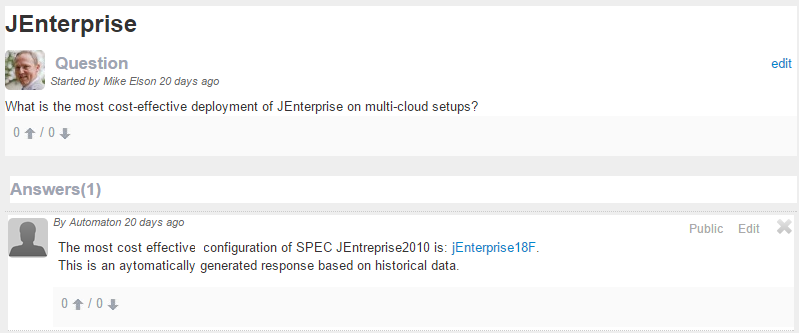
\includegraphics[scale=0.6]{./fig/nlp_example.png}
  \caption{Automated answer to user's question using NLP.}
  \label{fig:nlp_example}
\end{figure}

The automated replies provide the user with a direct possible answer to the question. So, it reduces the time waiting for an answer and provides a first helping hint about the user's question. If the answer is not efficient, other potential user of SNP can provide answers to the question and down-vote the automated reply.

Finally, a relevant question can be asked to the platform as ``Which deployments of JEnterprise provide the best performance for the lowest cost in a multi-cloud setup?''. This question is a paraphrased question of the previous one, talking about the same thing. The platform can find this similarity and provide the same automated answer.

\section{User interface}
This part of the thesis describes the User Interface of the Social Network Platform that is implementated based on 104 mock-ups created by HCI expert team. A mockup is a realistic representation of what the product will look like, in our case the Social Network Platform. The design of look \& feel of SNP is made by HCI expert team in order to follow the modern trends in Web Applications design. In order to support those look \& feel and the functionality of those mock-ups 25K lines of php, js and css code is written.
The key design objective of the social network platform is to create a strong bond between (i) software engineering services for managing and deploying cloud-targeted application models; and (ii) community-oriented facilities for communication and
collaboration between users. The interconnections between the two in the design of the user interface are depicted in Figure \ref{fig:two_aspects}.
The prototype implementation is publicly accessible on-line at http://socialnetwork.paasage.eu. 

\begin{figure}[h]
	\caption{The engineering \& social activities are seamlessly within the Platform.}
	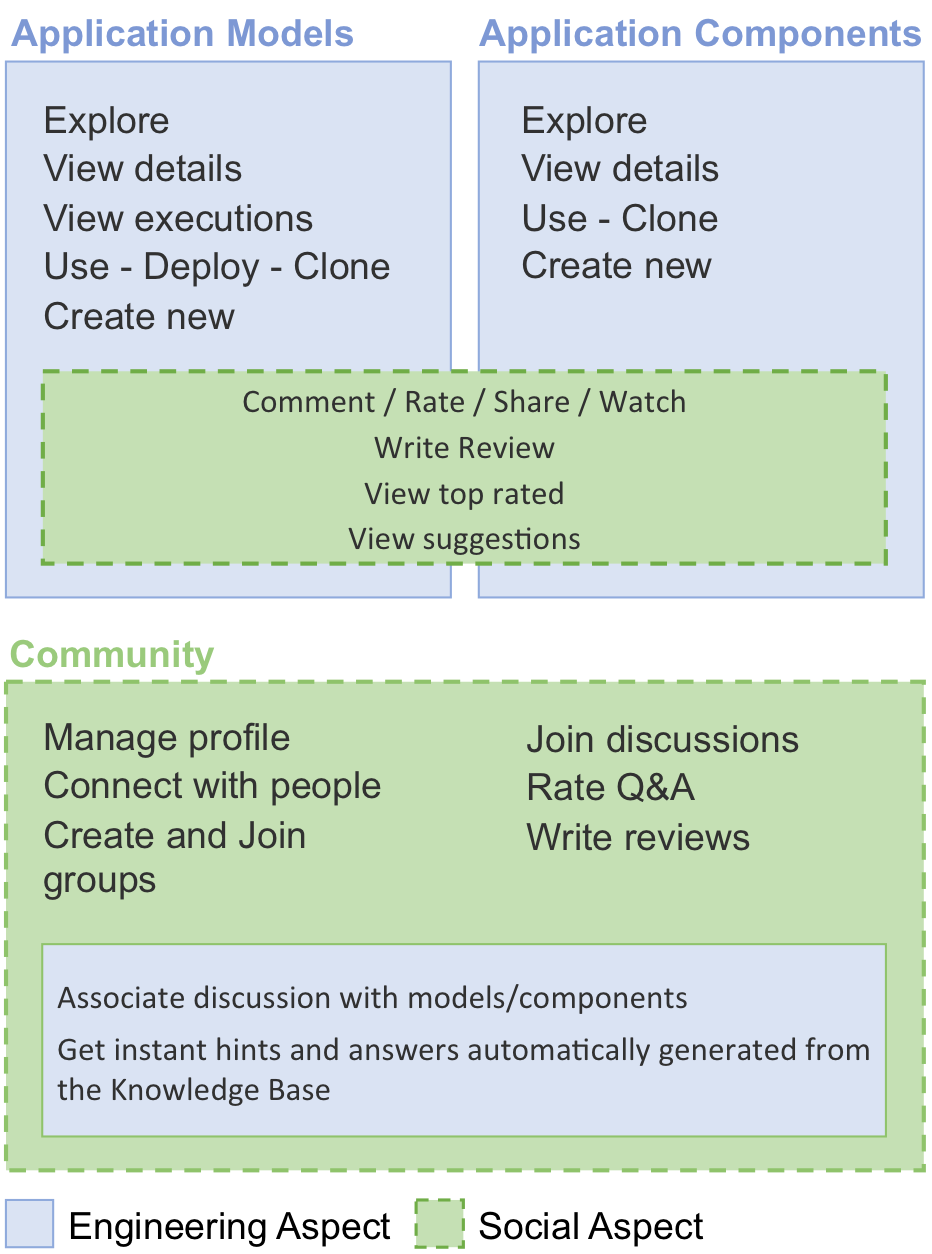
\includegraphics[width=0.6\textwidth,natwidth=200,natheight=150]{./fig/two_aspectes.png}
	\centering
	\label{fig:two_aspects}
\end{figure}

\subsection{User Interface Design Principles}
The discrete entities, which bind together the Social Networking with the application model aspects of Platform are:
\begin{itemize}
\item \emph{Application Models}. Application Models is a key entity of the platform. An example is shown if figure \ref{fig:jenter_home}, consisting of a human friendly description (label 1 in fig.\ref{fig:jenter_home}), the Camel Description of the model (label 2 in fig.\ref{fig:jenter_home}), reviews about the model (label 3 in fig.\ref{fig:jenter_home}). An overview of engineering aspects such as version and runs (label 4 in fig.\ref{fig:jenter_home}) and an overview of social aspects such as share and watch (label 5 in fig.\ref{fig:jenter_home}). The {\it share} action broadcast the model to the friends of the user that shares the model. The {\it watch} action notifies the user for future updates of the application model. 
\item \emph{Components}. We have integrated the Chef supermarket components into Social Network Platform. The components help the DevOps users to generate their application models as described in~\ref{sec:automatedcreation}. 
\item \emph{Users}. Users who basically are Cloud Deployment specialists and other users who want to know which deployment configuration they should use. Users can exchange knowledge to groups and benefit from the CAMEL repository. They can create or join groups, ask and answer questions, follow application models and create their own network of friends.
\item \emph{Groups}. As mentioned, every user of PaaSage Social Network Platform can create or join groups. Groups help users to interact with each other and gain knowledge from experts.
\end{itemize}

\begin{figure}[h]
	\caption{The application model home page}
	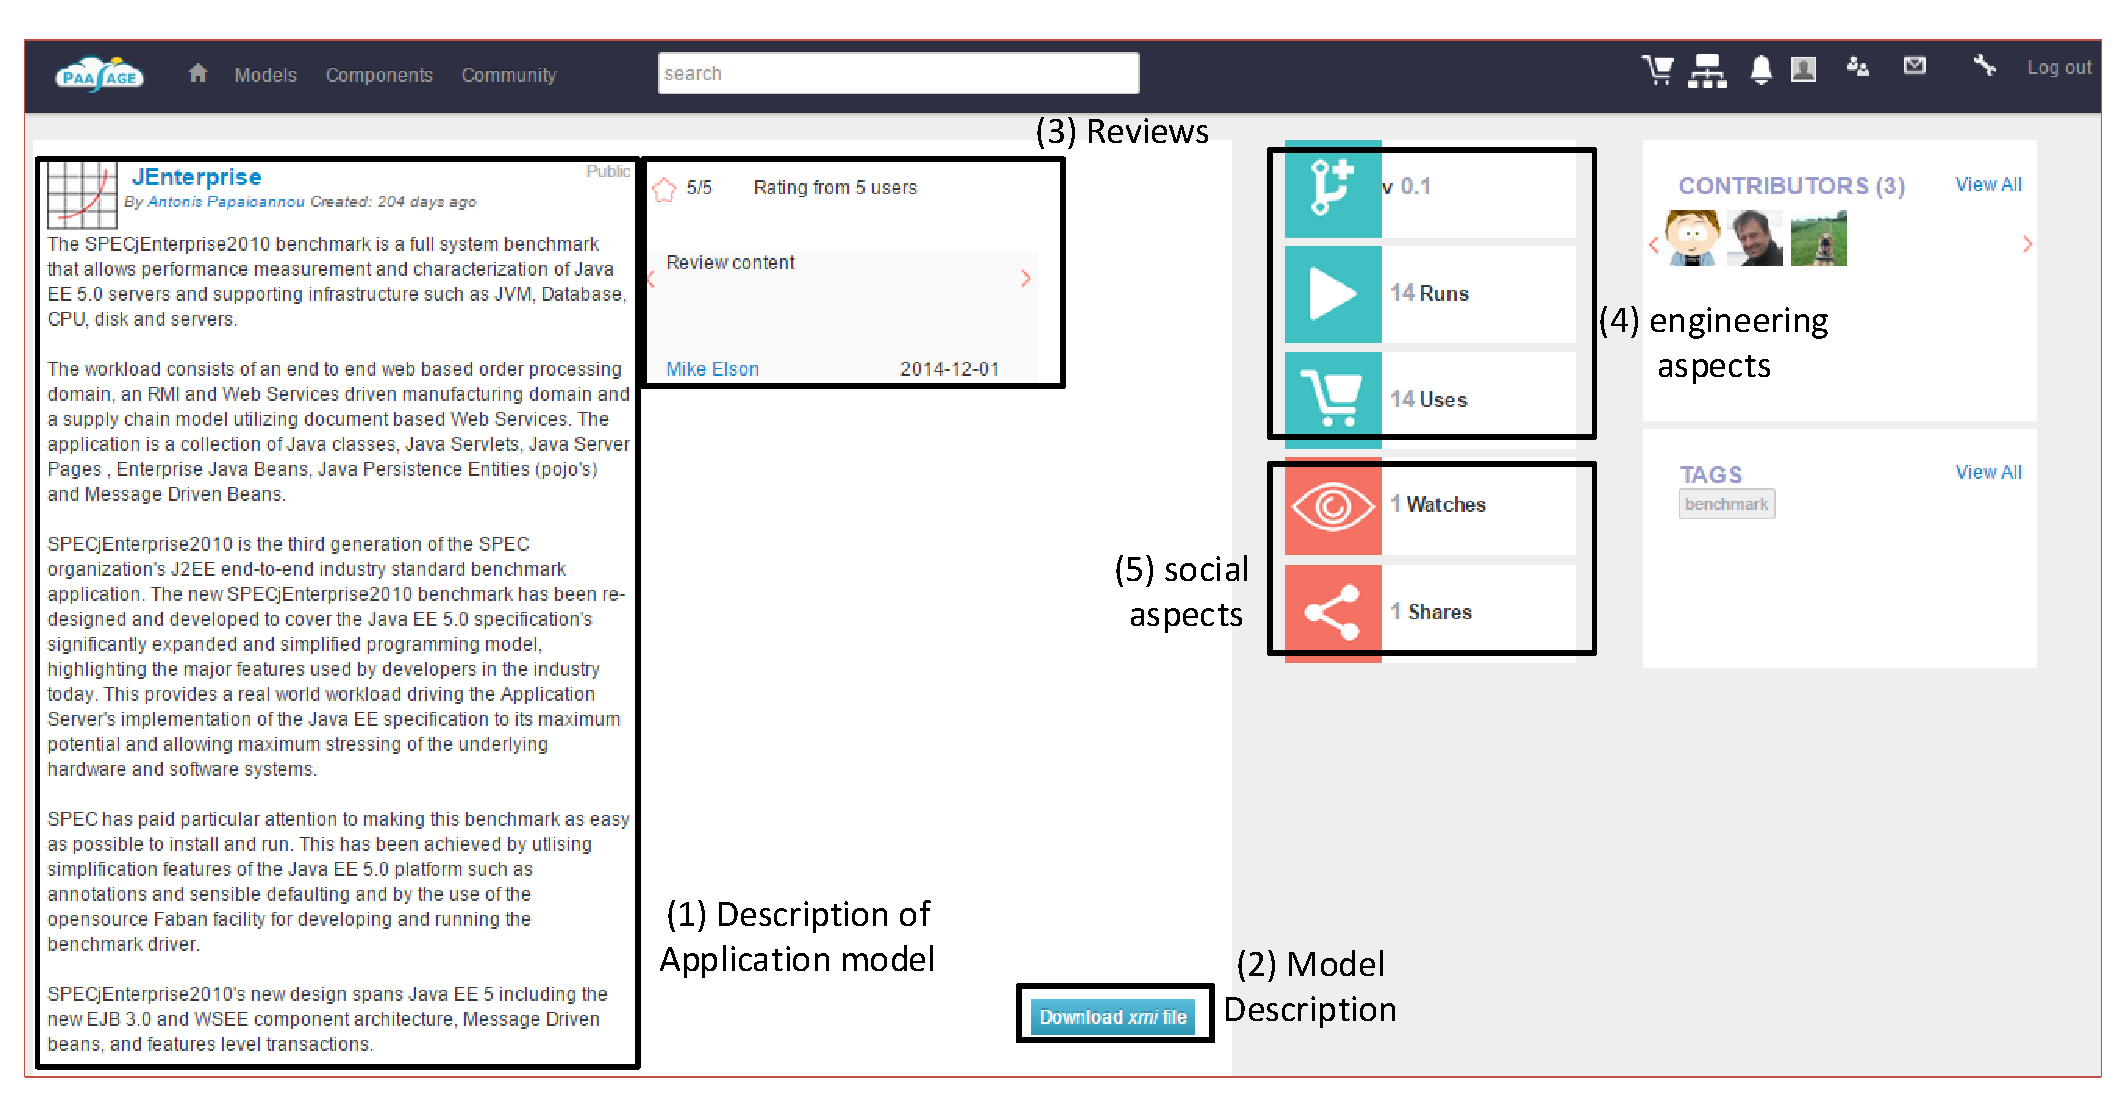
\includegraphics[width=1\textwidth,natwidth=200,natheight=150]{./fig/jenterprise_home_page.pdf}
	\centering
	\label{fig:jenter_home}
\end{figure}

\subsubsection{Gamification}
Following recent trends in social networks design and with the aim to motivate users active and regular participation in
the professional network, the design employs gamification features, meaning the use of video game elements in order to improve user experience and user engagement in non-game services and applications~\cite{deterding2011gamification}. One gamification feature in the Social Network design is the reward system for active community members. As users contribute content (models, components, ratings, reviews, questions, or answers) they receive experience points leading to special badges visible to all community members. Other features are the Profile completeness bar with suggestions on how to increase it. Finally, the concept of Model badges awarded to application and component models in case of excelling performance. Badges can serve among others as goal-setting devices, status symbols, and indications of reputation assessment procedures~\cite{antin2011badges}.

\section{Application Model Generation}
The DevOps users of PaaSage Social Network Platform can benefit from the automated creation of CAMEL baseline models presented at section~\ref{sec:automatedcreation} or upload their own created models using external editors like EMF~\cite{cdomodel} tree based editor or GMF~\cite{gmf_url} editor presented at section~\ref{sec:gmf}.

\subsection{Automated baseline Application Model Generation}
\label{sec:automatedcreation}
In order for users to create automated generated baseline CAMEL models, they can browse around the integrated Chef Components inside the Social Network and find the appropriate components for their applications. The platform has integrate a pointer for each Chef cookbook to the Social Network Database using the Chef Supermarket API~\cite{chef_api_url}. A PHP command has implemented in order to iterated through all Chef cookbooks and update the repository of SNP. This command has been configured and runs one time every day.

Through the Application Model Creation Page of the PaaSage Social Network Platform, the users can upload an external CAMEL model description of their application or create a new one with the help of the Platform in 4 simple steps as shown in figure ~\ref{fig:model_creation_0}. In the step zero~\ref{fig:sfig0}, the user is asked whether the new Application model already has an CAMEL model or whether the user wants to create a new Application CAMEL model through automated generation. For automated generation, the user must previously put the Chef cookbooks that he/she wants in the user's cart. The selected Chef cookbooks will be shown as a list of components. Then, in step one~\ref{fig:sfig1}, the user selects from this list which of the components will be included in the Application Model. 
In the example shown, the user has four components {\it mysqld}, {\it apache2}, {\it nodejs} and 
{\it ruby\_installer} and selects three of them. In the next step, shown in figure~\ref{fig:sfig2}, the user provides the deployment information (to which cloud provider the Application will run and which type of VMs will be used). Also, some components can be collocated in the same VM. In this example, the {\it nodejs} component will be collocated in the same VM as the {\it apache2}. In step tree, shown in figure~\ref{fig:sfig3}, the user provides the communication information between the components, for example the 
{\it nodejs} communicates with {\it mysqld} in the default mysql port {\it 3306}.

In the final step as shown in figure~\ref{fig:sfig4}, the user provides the final needed information about the name of the Application model, a human friendly description and the version of the model. In the bottom of the form of the figure~\ref{fig:sfig4} the user can find three actions: the \emph{Previous} action, the \emph{Save as draft} action and the \emph{Finalize} action. The \emph{Previous} action can performed all around the steps and make the user easily walk around the steps, giving him/her the opportunity to alter an option. The \emph{Save as draft} action creates the CAMEL model of the application but the model is not publicly available and only the creator or the contributors of the Application can see or edit the Model. The \emph{Finalize} action creates the CAMEL model of the application and makes it publicly available to the SNP users. 

For the creation of the base line CAMEL model an Ajax request is sent to a Java tool, that automatically creates the Application model according to the information that the user has already provided. When the Java tool generates the CAMEL model, it sends it back to the SNP. So the SNP can store this model to the repository. This tool is presented at~\cite{papoutsakis2014reducing}. 

\begin{figure}
\begin{subfigure}{.8\textwidth}
  \centering
  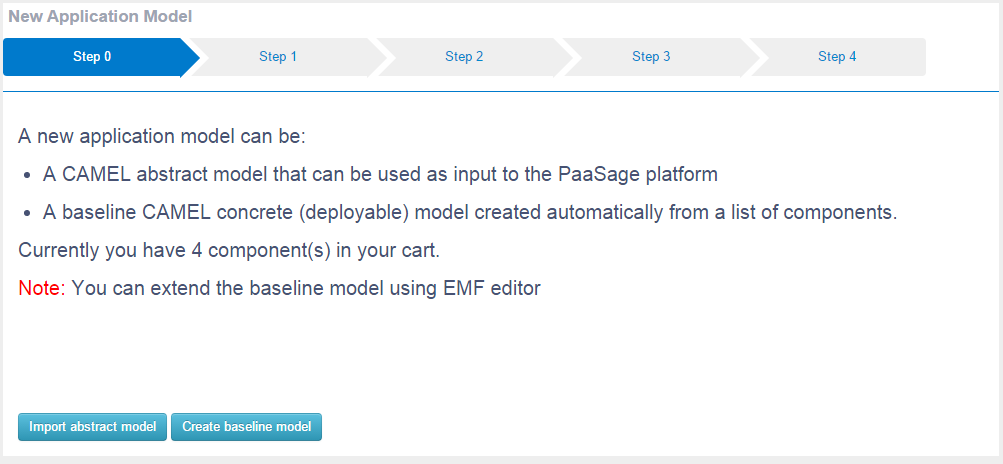
\includegraphics[scale=0.4]{./fig/model_creation0.png}
  \caption{Step 0: Upload external or create baseline model.}
  \label{fig:sfig0}
\end{subfigure} \\[1ex]
\begin{subfigure}{.8\textwidth}
  \centering
  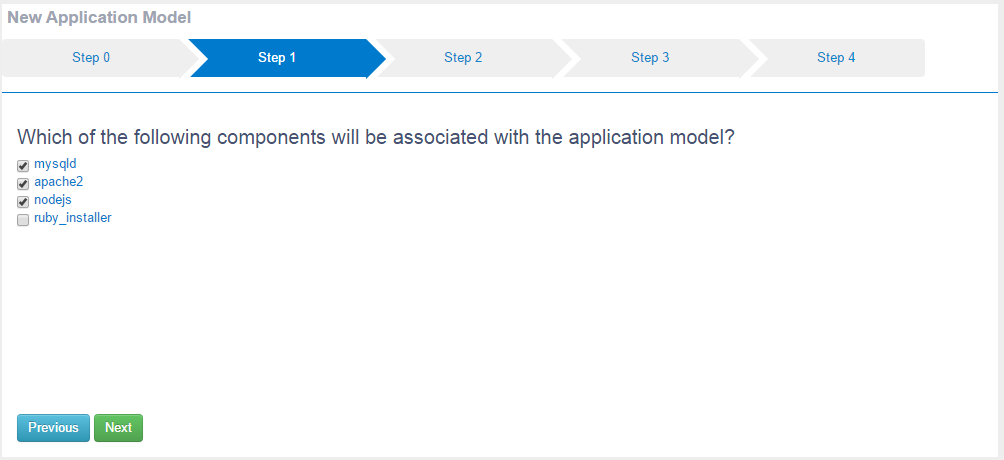
\includegraphics[scale=0.4]{./fig/model_creation1.png}
  \caption{Step 1: Choose the Components from the users' list.}
  \label{fig:sfig1}
\end{subfigure} \\[1ex]
\begin{subfigure}{.8\textwidth}
  \centering
  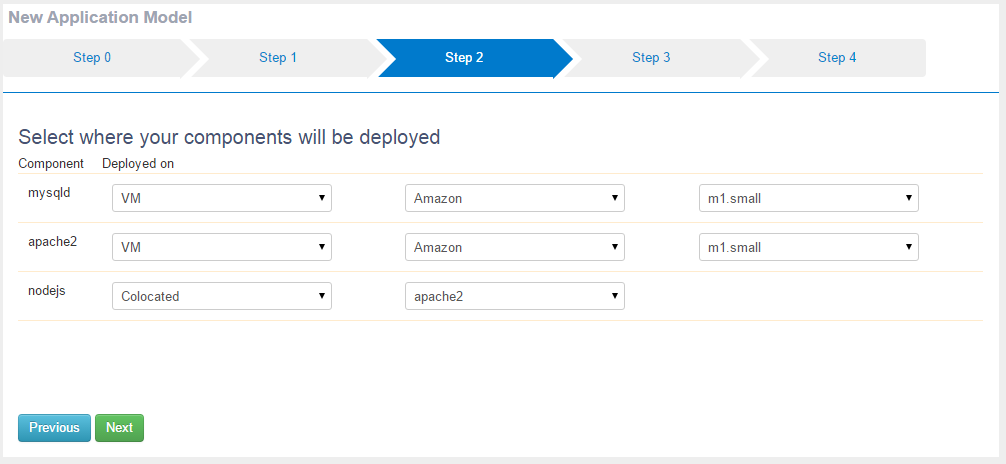
\includegraphics[scale=0.4]{./fig/model_creation2.png}
  \caption{Step 2: Deployment information.}
  \label{fig:sfig2}
\end{subfigure} \\[1ex]
\begin{subfigure}{.8\textwidth}
  \centering
  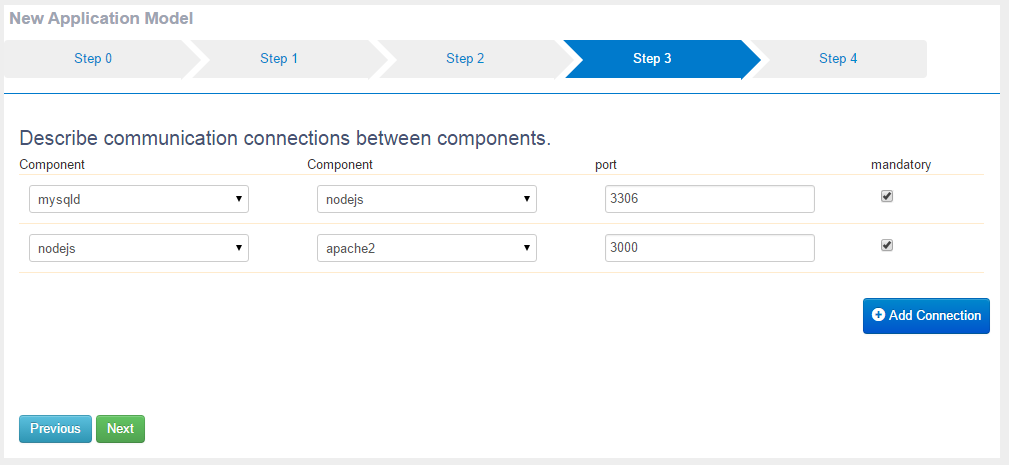
\includegraphics[scale=0.4]{./fig/model_creation3.png}
  \caption{Step 3: Communication Information.}
  \label{fig:sfig3}
\end{subfigure} \\[1ex]
\caption{Steps for Automated creation of baseline model.}
\label{fig:model_creation_0}
\end{figure}

\begin{figure}
  \centering
  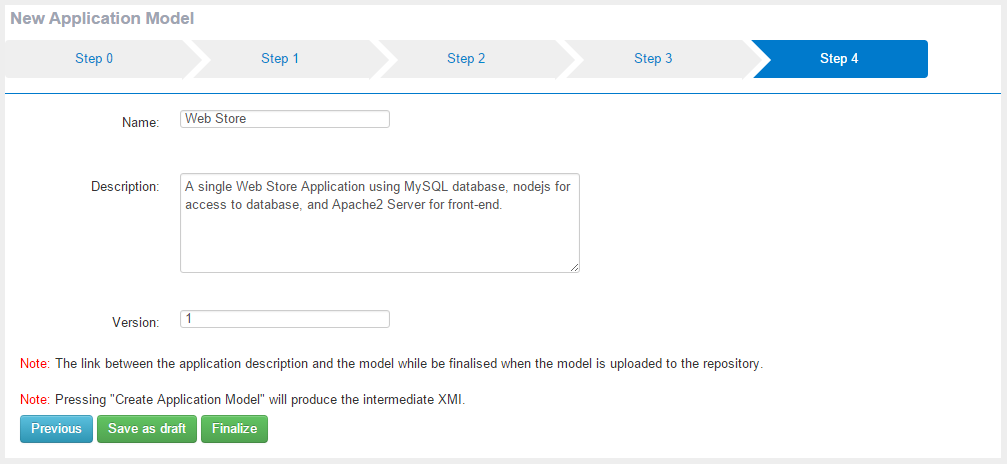
\includegraphics[scale=0.4]{./fig/model_creation4.png}
  \caption{Final Step of Automated creation of baseline model.}
  \label{fig:sfig4}
\end{figure}

\clearpage

\subsection{Graphical modeling of applications}
\label{sec:gmf}

Advanced users of the PaaSage Social Network Platform can compose application models through Graphical Modeling Framework (GMF)~\cite{gmf_url} which is an external Eclipse editor. GMF provides a set of generative components and runtime infrastructures for developing graphical editors based on Eclipse Modeling Framework (EMF) and Graphical Editing Framework (GEF). The GMF editor is generated from CAMEL {\em ecore} schema and provides the graphical palette to compose applications. 

Figure~\ref{fig:sensapp_as_gmf} shows the composition of a sample application model with the GMF editor. The palette in the right, contains all nodes and relationships needed to describe an application model. In the center, the composition of a sample application is shown, consisting of three VM types, the VM information about these VMs and the owner/user of the application. The GMF editor generates two files, one responsible for the graphical representation and the XMI description of the application model that can be uploaded to the social networking platform.

\begin{figure}
  \centering
  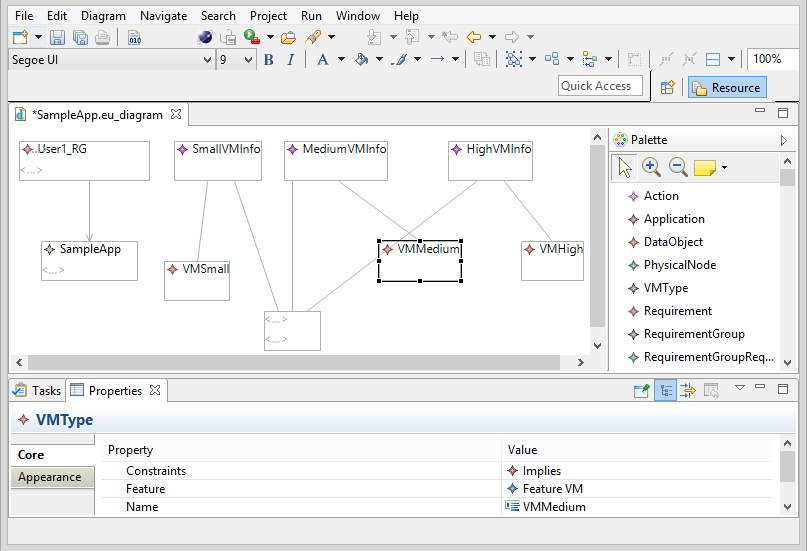
\includegraphics[scale=0.6]{./fig/gmf_editor.png}
  \caption{GMF editor composition of a sample application.}
  \label{fig:sensapp_as_gmf}
\end{figure}
